
\documentclass[a4paper,11pt]{jsarticle}
% !TEX encoding = UTF-8

\usepackage[dvipdfmx]{hyperref}
\usepackage{pxjahyper}


% 数式
\usepackage{amsmath,amsfonts}
\usepackage{bm}
\usepackage{physics}
\usepackage{amsmath,amssymb}
\usepackage{mathtools}
\numberwithin{equation}{section}

% 画像
\usepackage[dvipdfmx]{graphicx}
\usepackage{ascmac}

\usepackage{url}
\usepackage[dvipdfmx]{hyperref}

% \e と \i を定義
\providecommand{\e}{\mathrm{e}}
\renewcommand{\i}{\mathrm{i}}

\begin{document}

\title{エニオン}
\author{T.S.}
\date{\today}
\maketitle
\tableofcontents

以下の議論はNathan M. Myers "Thermodynamics of Statistic Anyons"による。\\

\section{Hong-Ou-Mandel効果}
HOM効果は量子光学で見つかった効果である。これを用いることによって、エニオニックな波動関数を作ることができる。\\
まず、HOM効果について復習しよう。2つのポートに、エンタングルしている光子のペアが対称的に入射する。
周波数や偏光状態などの自由度は同じとする。
初期状態がボソニックな空間部分の波動関数は、それぞれのインプットの重ね合わせで得られ、

\begin{align}
\ket{\psi_i^B}=\frac{1}{\sqrt{2}}(\ket{a}_1\ket{b}_2+\ket{b}_1\ket{a}_2)
\end{align}

となる。ビームスプリッタの作用は、状態を

\begin{align}
\ket{a}\to\frac{1}{\sqrt{2}}(\ket{c}+i\ket{d})\\
\ket{b}\to\frac{1}{\sqrt{2}}(i\ket{c}+\ket{d})
\end{align}

と変える。反射の際に、$\pi$の位相を獲得することが、変化の際の虚部に反映されていることに注意。
粒子のインデックスを追跡しながら、各インプットの状態についてこの発展を行うと、同じポートにいく状態のみが残ることがわかる:

\begin{align}
\ket{\psi_i^B}\to\ket{\psi_f^B}=\frac{i}{\sqrt{2}}(\ket{c}_1\ket{c}_2+\ket{d}_1\ket{d}_2)
\end{align}

物理的にはこれは有効的なボソン間の引力の現れとみれる(典型的には、”ボソンバンチング”と呼ばれる)。
\url{https://pc.watch.impress.co.jp/docs/news/yajiuma/754016.html} により、実験的にもわかっている。

\section{内部自由度を考慮したHOM効果}
フォトンの内部自由度を追加してHOM効果を拡張しよう。
フォトンをベル状態で用意することを考える。
4つの可能なベルペアは

\begin{align}
\ket{\Phi_A}=\frac{1}{\sqrt{2}}(\ket{00}+\ket{11})\\
\ket{\Phi_B}=\frac{1}{\sqrt{2}}(\ket{00}-\ket{11})\\
\ket{\Phi_C}=\frac{1}{\sqrt{2}}(\ket{01}+\ket{10})\\
\ket{\Phi_D}=\frac{1}{\sqrt{2}}(\ket{01}-\ket{10})\\
\end{align}

である。ここで、$\ket{0},\ket{1}$は直交する偏光状態である。
この追加の自由度を利用して、フェルミオンの、究極的にはエニオン的な統計量をフォトンにふるまいに組み込める。
このような使い方で、フォトンは”量子基板”と考えられる。\\
ここで、$\ket{\Phi_i},i=A,B,C$は対称的であり、$\ket{\Phi_D}$は反対称的であることに注意しよう。
フォトンはボソンであるから、全体の波動関数は対称的でなければならない。
よって、全体の波動関数としては2種類のパターンが考えられる。\\
ひとつめは

\begin{align}
  \ket{\Psi_i^B}=\frac{1}{\sqrt{2}}(\ket{a}_1\ket{b}_2+\ket{b}_1\ket{a}_2)\otimes\ket{\Phi_j},\,j=A,B,C
\end{align}

であり、ふたつめは

\begin{align}
  \ket{\Psi_i^F}=\frac{1}{\sqrt{2}}(\ket{a}_1\ket{b}_2-\ket{b}_1\ket{a}_2)\otimes\ket{\Phi_D}
\end{align}

である。無偏光状態を仮定すると、ビームスプリッタは波動関数の空間部分のみに作用する。
後者の場合、アウトプット状態は

\begin{align}
  \ket{\Psi_i^F}\to\ket{\Psi_f^F}=\frac{1}{\sqrt{2}}(\ket{c}_1\ket{d}_2-\ket{d}_1\ket{c}_2)
\end{align}

となり、フォトンのペアはお互いに異なるポートに向かうことになる。
これは有効的には、フェルミオン間の引力が働くということを示しており、パウリの排他律のあらわれであるとみれる。
フォトンは原理的にはボソンであるにもかかわらず、ビームスプリッタが反対称な部分のみにアクセスするため、フォトンはフェルミオンのようにふるまう。




\section{Hong-Ou-Mandel効果でエニオンの波動関数を作る}
このHOM効果は、対称or反対称のベル状態を調整することにより、エニオニックな統計に拡張できる。
偏光を回転させたビームスプリッタを使ったり、導波路を調整したり、偏光版を入れることにより、位相をコントロールできる。
対称と反対称にエンタングルしたペアを統計的に混ぜて用意してみよう:

\begin{align}
  \ket{\psi_i^A} = \frac{1}{\sqrt{2}} \left( \ket{a}_1 \ket{b}_2 + \mathrm{e}^{\i \pi \nu} \ket{b}_1 \ket{a}_2 \right)
\end{align}

これに対し、両方の光子が同じ方に来る確率は

\begin{align}
  P_{\mathrm{same}} &= |(\bra{c}_1\bra{c}_2+\bra{d}_1\bra{d}_2)\ket{\psi_f^A}|^2\\
  &=\frac{1}{2}[1+\cos(\pi \nu)] &&
\end{align}

と計算できる?(まだなってない。)\\
$\nu$ が様々な値をとるため、$P_{\mathrm{same}}$ は0から1まで値をとる。$N$個の光子をある割合で対称的にエンタングルさせ、残りは反対称にエンタングルさせたとする。
このときは、対称的or反対称的にエンタングルしているペアの分布をただ変えるだけでその振る舞いが反映される(平均的に)。
このフレームワークの中で、$\nu$はあるペアが対称的にエンタングルしている確率の尺度となる。すなわち、$\nu=\nu(p_B)$である。\\

\begin{itembox}[l]{\textbf{Def.エニオンの分類}}
多数のエニオンについて、統計的に$\nu=\nu(p_B)$の性質を持つエニオンを統計エニオンと呼ぶ。\\
対照的に、Wilczekの電荷と磁束の思考によるエニオンをトポロジカルエニオンと呼ぶ。したがって、分数量子ホール効果における準粒子励起もトポロジカルエニオンである。
\end{itembox}

多数ある粒子の平均として、ボソンとフェルミオンの中間のような性質をもつのが統計エニオンであって、準粒子そのものの性質として入れ替えの際に位相を得るのがトポロジカルエニオンであることに注意せよ。
また、トポロジカルエニオンといったときには、ここでは可換エニオンを考えることにする。可換エニオンとは、粒子の入れ替えにおいて単純に位相$\mathrm{e}^{i\pi\nu}$を得る粒子である。

トポロジーの立場に立てば、統計エニオンとトポロジカルエニオンの間には重要な区別が存在する。\\
トポロジカルエニオンの統計はブレイド(組みひも)群の表現である。(フェルミオンとボソンは置換群である。)
これは、2次元であることに起因しており、2回の粒子入れ替えが、何もしていないこととトポロジカルに区別しなくてはいけないというということである。
3次元では、2回の粒子入れ替えとなにもしないのとはトポロジカルに同等である。\\
これは物理的には、交換の方向が重要という結果を導く。2回同じ方向に入れ替えると、元の位相から$\mathrm{e}^{2i\pi \nu}$だけ変わる。\\
統計エニオンは、ボソンとフェルミオンの混合の平均であるから、2つの連続した交換は、交換の方向によらず、同じ波動関数に戻る。
混合の任意のペアをもってきたときの平均の位相はボソニックな位相とフェルミオニックな位相の平均である。すなわち、-1から1の間をとる。
ゆえに、位相$\mathrm{i\pi \nu}$をもつトポロジカルエニオンの混合に対応する統計エニオンは、混合の位相の平均が$cos(\pi \nu(p_B))$であるように重みづけされる。
我々は、可能なトポロジカルエニオンの位相を2次元空間を円とみる。ボソニックな位相とフェルミオニックな位相は正反対の位置として表現できる。
統計エニオンの平均された位相の可能な空間は、円の直径の線上で表現される。\\

この幾何学的な見方では、統計エニオンの平均された位相は対応するトポロジカルエニオンの位相の実数軸への角への射影とみなせる。(?)
図2がこの見方の図である。
この比較から、ブレイド群の表現として、トポロジカルエニオンは統計エニオンより複雑であることがわかる。
ここで、トポロジカルエニオンと統計エニオンの熱力学的な性質はどのように異なるか気になるだろう。から、次からその話を始めよう。

\section{統計エニオンの波動関数}
量子光学での知見から、統計エニオンを考えてみる。ボソニックな粒子のペアの波動関数の空間部分(内部自由度を除いた部分のこと)は

\begin{align}
\Psi_B(x,y) = \frac{1}{\sqrt{2(1+\delta_{n_1,n_2})}}[\psi_{n1}(x)\psi_{n2}(y)+\psi_{n1}(y)\psi_{n2}(x)]
\end{align}

ここで$\psi_n(x)$は量子数$n$に対応する規格化された1粒子固有状態である。規格化係数は、2粒子が同じときと違うときで変わる。区別できる2粒子のとき、因子2がかかる。
これは古典的な場合にかかる因子と同じである。
同様にフェルミオニックな波動関数は

\begin{align}
  \Psi_F(x,y) = \frac{1}{\sqrt{2}}[\psi_{n1}(x)\psi_{n2}(y)-\psi_{n1}(y)\psi_{n2}(x)]
\end{align}

フェルミオニックな波動関数のときは、規格化係数に$\delta$関数は必要ない。←これはなぜ?\\
$N$個の独立な粒子のペアについて、$N_B$個のペアが交換の際に対称的で、$N-N_B$個が反対称的であるとすると、

\begin{align}
\Psi(\vb*{x_1},\vb*{x_2},...,\vb*{x_N})=\prod_{j=1}^{N_B}\Psi_B(\vb*{x}_j)\prod_{k=N_B+1}^{N}\Psi_F(\vb*{x}_k)
\end{align}

となる。ここで、$\vb*{x_i}=(x,y)$である。
そしてこれは、統計エニオンの枠組みにおいて、次の式と等価である:

\begin{align}
  \Psi(\vb*{x_1},\vb*{x_2},...,\vb*{x_N})=\prod_{j=1}^{N}\Psi_A(\vb*{x}_j)
\end{align}

ここで、

\begin{align}
\Psi_A(\vb*{x}_j)=\frac{1}{\sqrt{2(1+\delta_{n_1,n_2})}}[\psi_{n1}(x_j)\psi_{n2}(y_j)+\mathrm{e}^{i\pi\nu_j}\psi_{n1}(y_j)\psi_{n2}(x_j)]
\end{align}

である。これをみると、統計エニオンは1粒子波動関数の積から成り立っていることがわかる。一方、トポロジカルエニオンの波動関数は一般に、エニオニックな位相のボソニック、フェルミオニックな極限を除いて、一粒子波動関数の積にはならないことに注意。
統計エニオンの波動関数内の積は、$N_B$個の対称な波動関数と$N_F$個の波動関数を与えなければならない。
この条件は、$\nu_j=\Theta(j-N_B-1)$となるとき満たされる。ここで、$\Theta(・)$はHeavisideの階段関数である。$\Theta(0)=1$としている。
このフレームワークでは、$\Psi_A(\vb*{x}_j)$のエニオニックな位相因子($\mathrm{e}^{i\pi\nu_j}$)は$N$個の粒子のペアのあらゆる交換の平均として考えられる。
大きな$N$については、$N_B=Np_B,N_F=N(1-p_B)$として表現できる。ここで、$p_B(p_F)$はペアがボソニック(フェルミオニック)な位相を持つ確率である。
この章の最後に、2粒子系の極限を考えてみよう。このとき、エニオニックな波動関数は

\begin{align}
  \Psi_A(\vb*{x})=\frac{1}{\sqrt{2(1+\delta_{n_1,n_2})}}[\psi_{n1}(x)\psi_{n2}(y)\pm \psi_{n1}(y)\psi_{n2}(x)]
\end{align}

ここで、符号は$p_B$が0か1かで決まる。個々のペアはボソンかフェルミオンかのどちらかであるということを反映している。

\section{統計エニオンの第二量子化}
適切な交換関係を決めることによって、統計エニオンは第二量子化をすることができる。

\subsection{トポロジカルエニオンの第二量子化}
まずトポロジカルエニオンについて考えよう。トポロジカルエニオンの生成消滅演算子については、ボソニックまたはフェルミオニックな演算子のJordan-Wigner変換(なんだこれ?)から作られる:
\\

\begin{itembox}[l]{\textbf{Def.トポロジカルエニオンの生成消滅演算子 }}
$\mathcal{C}$を交換のために回す方向で考える閉曲線とする。$a(\vb*{x}_\mathcal{C}),a^{\dag}(\vb*{x}_\mathcal{C})$を$\mathcal{C}$に沿った$\vb*{x}$の消滅,生成演算子とする。
このとき、トポロジカルエニオンの交換関係は次で与えられる。
\begin{align}
a(\vb*{x}_\mathcal{C})a(\vb*{y}_\mathcal{C})-\mathrm{e}^{-i\pi\nu}a(\vb*{y}_\mathcal{C})a(\vb*{x}_\mathcal{C})=0\\
a(\vb*{x}_\mathcal{C})a^{\dag}(\vb*{y}_\mathcal{C})-\mathrm{e}^{i\pi\nu}a^{\dag}(\vb*{y}_\mathcal{C})a(\vb*{x}_\mathcal{C})=0\\
a^{\dag}(\vb*{x}_\mathcal{C})a(\vb*{y}_\mathcal{C})-\mathrm{e}^{i\pi\nu}a(\vb*{y}_\mathcal{C})a^{\dag}(\vb*{x}_\mathcal{C})=0\\
a^{\dag}(\vb*{x}_\mathcal{C})a^{\dag}(\vb*{y}_\mathcal{C})-\mathrm{e}^{-i\pi\nu}a^{\dag}(\vb*{y}_\mathcal{C})a^{\dag}(\vb*{x}_\mathcal{C})=0
\end{align}
\end{itembox}

すなわち、生成同士、消滅同士の交換にはマイナスの位相がかかり、生成と消滅の交換にはプラスの位相がかかる。
トポロジカルエニオンの演算子はブレイド群の表現であるから、交換は時計回りか反時計回りかに依存する。(図1を参照。)
\begin{figure}[htbp]
\begin{center}
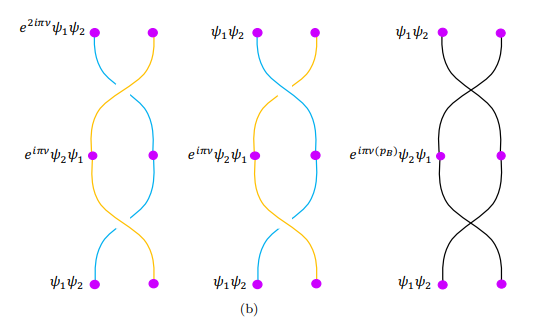
\includegraphics[width=100mm]{anyonwf.png}
\caption{ブレイド}
\end{center}
\end{figure}

交換関係を見ると、$\nu=0$でボソンの交換関係を、$\nu=1$でフェルミオンの交換関係を復元することがわかる。
とくに、同じ位置にある粒子においては、エニオニックな位相はキャンセルされ、正準交換関係に帰着する:
\begin{align}
  a(\vb*{x}_\mathcal{C})a^{\dag}(\vb*{x}_\mathcal{C})\pm a^{\dag}(\vb*{x}_\mathcal{C})a(\vb*{x}_\mathcal{C})=1\\
\end{align}
ここで、エニオニックな演算子がフェルミオニックな演算子からきている場合は+、ボソニックな演算子からきている場合は$-$をとる。\\
一般に、トポロジカルエニオンは、$\nu\neq0$のとき、”ハードコアボソン”としてふるまう。ハードコアボソンとは、同じ位置にいない(排他律のある)ボソンである。
この意味で、$\nu$は2つの同一粒子の間の斥力の自由度を定量化していると考えられる。\\
ここの議論は\url{https://www.sciencedirect.com/science/article/pii/055032139390316H}{ A.Lerda, S.Sciuto. Anyons and Quantum Groups}による。

ハードコアボソンの生成消滅演算子$c_i^{\dag}(x_C),c_i(x_C)$を用いて、その議論を追ってみたい。
\begin{align}
  a(\vb*{x}_\mathcal{C})a^{\dag}(\vb*{x}_\mathcal{C})&=K_i(\vb*{x}_C)c_i(\vb*{x})c_i^{\dag}(\vb*{x})K_i^{\dag}(\vb*{x}_C)\\
  &=K_i(\vb*{x}_C)(-c_i^{\dag}(\vb*{x})c_i(\vb*{x})+1)K_i^{\dag}(\vb*{x}_C)\\
  &=-\mathrm{e}^{i\nu\Theta_C(\vb*{x},\vb*{x})}c_i^{\dag}(\vb*{x})K_i(\vb*{x}_c)\mathrm{e}^{i\nu\Theta_C(\vb*{x},\vb*{x})}K_i^{\dag}c_i(\vb*{x})+1\\
  &=-a_i^{\dag}(\vb*{x}_C)a_i(\vb*{x}_C)+1
\end{align}
ただし、
\begin{align}
 K_i(\vb*{x}_C)&=\mathrm{exp}(i\nu\sum_{y\in\Omega}\Theta_{c_{\vb*{x}}}(x,y)c_i^{\dag}(y)c_i(y))\\
K_i^{\dag}(\vb*{x}_C)&=c.c.=K_i^{-1}(\vb*{x}_c)
\end{align}
は、disorder演算子と呼ばれるものである。$\Omega,\Theta$はあとで定義を書くことにする。
これにより中途半端に示された。

\subsection{統計エニオンの第二量子化}
では次に、統計エニオンについて考えよう。
統計エニオンの生成消滅演算子を考えるには、統計エニオンの波動関数を構成したときを思い出せばよい。
量子多体系のHilbert空間として、Fock空間を考える。
そうすると、
\begin{align}
\ket{1}_1\ket{1}_2\dots\ket{1}_N=\prod _{j=1}^{N_B}b_j^{\dag}\ket{0}_j\prod _{k=N_B+1}^{N}f_k^{\dag}\ket{0}_k
\end{align}
と書くことができる。これと同等の表現として統計エニオンの生成演算子を考える:
\begin{align}
  \ket{1}_1\ket{1}_2\dots\ket{1}_N=\prod _{j=1}^{N}s_j^{\dag}\ket{0}_j
\end{align}
演算子$s_j^{\dag}$は、$j\leq N_B$ではボソンの生成演算子に、$N_B\leq j$ではフェルミオンの生成演算子にならなくてはならない。
同様に、消滅演算子も同じ条件を満たさなくてはならない。
この制限のもと、統計エニオンの交換関係は以下のようになる:\\

\begin{itembox}[l]{\textbf{Def.統計エニオンの交換関係 }}
  統計エニオンの交換関係は
\begin{align}
s_j^{\dag}s_j-\mathrm{e}^{i\pi\Theta(j-N_B-1)}s_j s_j^{\dag}=1\\
s_js_j^{\dag}-\mathrm{e}^{i\pi\Theta(j-N_B-1)}s_j^{\dag} s_j=1\\
s_j^{\dag}s_j^{\dag}-\mathrm{e}^{i\pi\Theta(j-N_B-1)}s_j^{\dag} s_j^{\dag}=0\\
s_js_j-\mathrm{e}^{i\pi\Theta(j-N_B-1)}s_j s_j=0
\end{align}
と定義する。
\end{itembox}

1粒子極限を考えると、生成演算子と消滅演算子の関係は

\begin{align}
s_js_j^{\dag}\pm s_j^{\dag}s_j=1
\end{align}

に帰着する。これは、現実にはボソンかフェルミオンかのどちらかであるということを反映している。
また、これは、(5)式の交換関係がフェルミオニックな演算子を元に作られたか、ボソニックな演算子を元に作られたかに依存することを反映している。

\section{統計エニオンと一般化排他統計(Generalized Exclusion Statistics)}
統計エニオンのフェルミオン極限を除いて、統計エニオンとトポロジカルエニオンの注目すべき違いは、排他律がないことである。
かわりに、統計エニオンは”部分的に占有された”状態を許す。
”部分的に占有された状態”というのは、全系の占有率が平均以上の状態である(?)。
この意味で、統計エニオンのフレームワークというのはHaldaneの一般化排他統計(Generalized Exclusion Statistics,GES)に似ている。\\
GESはパウリの排他律を拡張することによって作られたものである。
粒子数を変化させるもとで、量子系のHilbert空間の次元の変化を定量化するパラメタライズされた差分関係(differential relation)を定義することにより拡張された。(この文はまだよくわかっていないのでこんな感じ)
差分関係は

\begin{align}
\Delta  d_{GES}=-g \Delta  N
\end{align}

である。ここで左辺は次元の変化であり、$g$はパラメータだと考えられる。\\
ボソンに対しては、同じ状態を占められる粒子数は無限であるから、次元は粒子数に依存しない。よって$g=0$である。\\
フェルミオンに対しては、排他律のために、それぞれ、追加される粒子によって直接的に次元がスケールされる(粒子がいない次元は考えなくてよいということ?)。よって$g=1$である。\\
GES統計エニオンは、相互作用する気体、たとえばCalogero-Sutherlandモデルなどで見られることが示されている。
驚くべきことに、このGESエニオンの実現は、最低Landau準位に閉じ込められたトポロジカルエニオンに直接マッピングできる。
GESエニオンは、極低温Hubberdチェインと同様に、Calogero-SutherlandモデルやLieb-Linigerモデル、ハードコアTonks-Girardeau気体などに見られている。
もっと一般に、GESに従う理想準粒子の観点から、熱力学的Bethe仮設によって計算しなおせる可積分モデルの存在が示されている。\\
この統計エニオンのフレームワークでは、統計エニオンのHilbert空間の次元変化はボソンの次元変化とフェルミオンの次元変化の和で与えられる。
それぞれの出現確率$p_B,p_F$を用いて、
\begin{align}
\Delta d_{SA}=p_B\Delta d_b+p_F\Delta d_F
\end{align}
とかける。
$\Delta d_B=0,\Delta d_F=-\Delta N$のとき、$\Delta d_{SA}=-p_F\Delta N$と単純になる。
はじめの式と一つ上の式を見比べると、GESのフレームワークにおけるパラメータ$g$というのは、統計エニオンのフレームワークにおけるフェルミオンの出現確率によってきまってしまうということがわかる。
これは統計エニオンのフレームワークがGESエニオンのフレームワークとまったく同等であることを示している。
GESエニオンはボソンとフェルミオンの観点から説明できることは、MurthyとShankerが、Calogero-Sutherlandモデルは理想GESエニオンであることを指摘した際にわかった。
その結果、分配関数はボソニックな部分とフェルミオニックな部分に分けられ、それぞれ、GESパラメータ$g,g-1$の累乗で構成されることがわかった。
これにより、GESはボソンとフェルミオンの理想敵な混合であることが指摘された。\\
統計エニオン、GESエニオンは任意の次元で実現できる(次元に一般的な制限はない)というのは、トポロジカルエニオンとの大きな違いである。


\section{エニオンの平衡熱力学}
\subsection{1次元統計エニオン}
エニオン系の熱力学を理解するためにまず考えることは、熱力学量にエニオンの位相がどのように依存するかである。
これをきめるために、適切な分配関数を導入する。トラップされた相互作用するGESガスの実現でモチベートされたように、1次元調和ポテンシャル中の2つの統計エニオンを考えよう。\\
しかし、この際、我々は相互作用しない粒子系を考えている。
(GESは単なる混合でよいのか?)
トラップされたボソンーフェルミオン混合物は以前より、理論的あるいは実験的に研究されているが、この研究ではおもに、基底状態の設定でボソン、フェルミオン間の相互作用から生じる効果に焦点を当てよう。
統計エニオンのフレームワークでは我々は、混合物の代わりに、そのような混合の理想気体極限として多体平均のふるまいを考える。
調和ポテンシャル中に閉じ込められた2つの統計エニオンのハミルトニアンは

\begin{align}
H=\frac{p_1^2+p_2^2}{2m}+\frac{1}{2}m\omega^2(x_1^2+x_2^2)
\end{align}
で与えられる。統計エニオンののフレームワークでは、ハミルトニアンのもとで発展するエニオンのペアの分配関数というのは
\begin{align}
Z_{SA}=(Z_B)^{p_B}(Z_F)^{1-p_B}
\end{align}
となる。ここで、それぞれの粒子の分配関数を$Z_i,i=B,F$とした。元論文の付録Aにはこの分配関数の導き方が書いてあるので余裕があるときに読む。
この分配関数は、CSmodelの$g\rightarrow1-p_B$としたものに等しい。
我々はここに、統計エニオンの枠組みの中では、エニオニックなふるまいというのは、ハミルトニアンの中の相互作用項からというよりむしろ、平均の性質の上で純粋に現れるのである。(CSmodelをもっと見てみる必要があるよこれは)
この分配関数を使うと、熱力学的な量はただちに導かれる。
分配関数を実際に代入してみると、

\begin{align}
E=\frac{1}{2}\hbar \omega[3\coth (\beta\hbar\omega)+\csch(\beta\hbar\omega)-2p_B+1 ]
\end{align}





\end{document}

=======
\documentclass[a4paper,11pt]{jsarticle}
% !TEX encoding = UTF-8

\usepackage[dvipdfmx]{hyperref}
\usepackage{pxjahyper}


% 数式
\usepackage{amsmath,amsfonts}
\usepackage{bm}
\usepackage{physics}
\usepackage{amsmath,amssymb}
\usepackage{mathtools}
\numberwithin{equation}{section}

% 画像
\usepackage[dvipdfmx]{graphicx}
\usepackage{ascmac}

\usepackage{url}
\usepackage[dvipdfmx]{hyperref}

% \e と \i を定義
\providecommand{\e}{\mathrm{e}}
\renewcommand{\i}{\mathrm{i}}

\begin{document}

\title{エニオン}
\author{T.S.}
\date{\today}
\maketitle
\tableofcontents

以下の議論はNathan M. Myers "Thermodynamics of Statistic Anyons"による。\\

\section{Hong-Ou-Mandel効果}
HOM効果は量子光学で見つかった効果である。これを用いることによって、エニオニックな波動関数を作ることができる。\\
まず、HOM効果について復習しよう。2つのポートに、エンタングルしている光子のペアが対称的に入射する。
周波数や偏光状態などの自由度は同じとする。
初期状態がボソニックな空間部分の波動関数は、それぞれのインプットの重ね合わせで得られ、

\begin{align}
\ket{\psi_i^B}=\frac{1}{\sqrt{2}}(\ket{a}_1\ket{b}_2+\ket{b}_1\ket{a}_2)
\end{align}

となる。ビームスプリッタの作用は、状態を

\begin{align}
\ket{a}\to\frac{1}{\sqrt{2}}(\ket{c}+i\ket{d})\\
\ket{b}\to\frac{1}{\sqrt{2}}(i\ket{c}+\ket{d})
\end{align}

と変える。反射の際に、$\pi$の位相を獲得することが、変化の際の虚部に反映されていることに注意。
粒子のインデックスを追跡しながら、各インプットの状態についてこの発展を行うと、同じポートにいく状態のみが残ることがわかる:

\begin{align}
\ket{\psi_i^B}\to\ket{\psi_f^B}=\frac{i}{\sqrt{2}}(\ket{c}_1\ket{c}_2+\ket{d}_1\ket{d}_2)
\end{align}

物理的にはこれは有効的なボソン間の引力の現れとみれる(典型的には、”ボソンバンチング”と呼ばれる)。
\url{https://pc.watch.impress.co.jp/docs/news/yajiuma/754016.html} により、実験的にもわかっている。

\section{内部自由度を考慮したHOM効果}
フォトンの内部自由度を追加してHOM効果を拡張しよう。
フォトンをベル状態で用意することを考える。
4つの可能なベルペアは

\begin{align}
\ket{\Phi_A}=\frac{1}{\sqrt{2}}(\ket{00}+\ket{11})\\
\ket{\Phi_B}=\frac{1}{\sqrt{2}}(\ket{00}-\ket{11})\\
\ket{\Phi_C}=\frac{1}{\sqrt{2}}(\ket{01}+\ket{10})\\
\ket{\Phi_D}=\frac{1}{\sqrt{2}}(\ket{01}-\ket{10})\\
\end{align}

である。ここで、$\ket{0},\ket{1}$は直交する偏光状態である。
この追加の自由度を利用して、フェルミオンの、究極的にはエニオン的な統計量をフォトンにふるまいに組み込める。
このような使い方で、フォトンは”量子基板”と考えられる。\\
ここで、$\ket{\Phi_i},i=A,B,C$は対称的であり、$\ket{\Phi_D}$は反対称的であることに注意しよう。
フォトンはボソンであるから、全体の波動関数は対称的でなければならない。
よって、全体の波動関数としては2種類のパターンが考えられる。\\
ひとつめは

\begin{align}
  \ket{\Psi_i^B}=\frac{1}{\sqrt{2}}(\ket{a}_1\ket{b}_2+\ket{b}_1\ket{a}_2)\otimes\ket{\Phi_j},\,j=A,B,C
\end{align}

であり、ふたつめは

\begin{align}
  \ket{\Psi_i^F}=\frac{1}{\sqrt{2}}(\ket{a}_1\ket{b}_2-\ket{b}_1\ket{a}_2)\otimes\ket{\Phi_D}
\end{align}

である。無偏光状態を仮定すると、ビームスプリッタは波動関数の空間部分のみに作用する。
後者の場合、アウトプット状態は

\begin{align}
  \ket{\Psi_i^F}\to\ket{\Psi_f^F}=\frac{1}{\sqrt{2}}(\ket{c}_1\ket{d}_2-\ket{d}_1\ket{c}_2)
\end{align}

となり、フォトンのペアはお互いに異なるポートに向かうことになる。
これは有効的には、フェルミオン間の引力が働くということを示しており、パウリの排他律のあらわれであるとみれる。
フォトンは原理的にはボソンであるにもかかわらず、ビームスプリッタが反対称な部分のみにアクセスするため、フォトンはフェルミオンのようにふるまう。




\section{Hong-Ou-Mandel効果でエニオンの波動関数を作る}
このHOM効果は、対称or反対称のベル状態を調整することにより、エニオニックな統計に拡張できる。
偏光を回転させたビームスプリッタを使ったり、導波路を調整したり、偏光版を入れることにより、位相をコントロールできる。
対称と反対称にエンタングルしたペアを統計的に混ぜて用意してみよう:

\begin{align}
  \ket{\psi_i^A} = \frac{1}{\sqrt{2}} \left( \ket{a}_1 \ket{b}_2 + \mathrm{e}^{\i \pi \nu} \ket{b}_1 \ket{a}_2 \right)
\end{align}

これに対し、両方の光子が同じ方に来る確率は

\begin{align}
  P_{\mathrm{same}} &= |(\bra{c}_1\bra{c}_2+\bra{d}_1\bra{d}_2)\ket{\psi_f^A}|^2\\
  &=\frac{1}{2}[1+\cos(\pi \nu)] &&
\end{align}

と計算できる?(まだなってない。)\\
$\nu$ が様々な値をとるため、$P_{\mathrm{same}}$ は0から1まで値をとる。$N$個の光子をある割合で対称的にエンタングルさせ、残りは反対称にエンタングルさせたとする。
このときは、対称的or反対称的にエンタングルしているペアの分布をただ変えるだけでその振る舞いが反映される(平均的に)。
このフレームワークの中で、$\nu$はあるペアが対称的にエンタングルしている確率の尺度となる。すなわち、$\nu=\nu(p_B)$である。\\

\begin{itembox}[l]{\textbf{Def.エニオンの分類}}
多数のエニオンについて、統計的に$\nu=\nu(p_B)$の性質を持つエニオンを統計エニオンと呼ぶ。\\
対照的に、Wilczekの電荷と磁束の思考によるエニオンをトポロジカルエニオンと呼ぶ。したがって、分数量子ホール効果における準粒子励起もトポロジカルエニオンである。
\end{itembox}

多数ある粒子の平均として、ボソンとフェルミオンの中間のような性質をもつのが統計エニオンであって、準粒子そのものの性質として入れ替えの際に位相を得るのがトポロジカルエニオンであることに注意せよ。
また、トポロジカルエニオンといったときには、ここでは可換エニオンを考えることにする。可換エニオンとは、粒子の入れ替えにおいて単純に位相$\mathrm{e}^{i\pi\nu}$を得る粒子である。

トポロジーの立場に立てば、統計エニオンとトポロジカルエニオンの間には重要な区別が存在する。\\
トポロジカルエニオンの統計はブレイド(組みひも)群の表現である。(フェルミオンとボソンは置換群である。)
これは、2次元であることに起因しており、2回の粒子入れ替えが、何もしていないこととトポロジカルに区別しなくてはいけないというということである。
3次元では、2回の粒子入れ替えとなにもしないのとはトポロジカルに同等である。\\
これは物理的には、交換の方向が重要という結果を導く。2回同じ方向に入れ替えると、元の位相から$\mathrm{e}^{2i\pi \nu}$だけ変わる。\\
統計エニオンは、ボソンとフェルミオンの混合の平均であるから、2つの連続した交換は、交換の方向によらず、同じ波動関数に戻る。
混合の任意のペアをもってきたときの平均の位相はボソニックな位相とフェルミオニックな位相の平均である。すなわち、-1から1の間をとる。
ゆえに、位相$\mathrm{i\pi \nu}$をもつトポロジカルエニオンの混合に対応する統計エニオンは、混合の位相の平均が$cos(\pi \nu(p_B))$であるように重みづけされる。
我々は、可能なトポロジカルエニオンの位相を2次元空間を円とみる。ボソニックな位相とフェルミオニックな位相は正反対の位置として表現できる。
統計エニオンの平均された位相の可能な空間は、円の直径の線上で表現される。\\

この幾何学的な見方では、統計エニオンの平均された位相は対応するトポロジカルエニオンの位相の実数軸への角への射影とみなせる。(?)
図2がこの見方の図である。
この比較から、ブレイド群の表現として、トポロジカルエニオンは統計エニオンより複雑であることがわかる。
ここで、トポロジカルエニオンと統計エニオンの熱力学的な性質はどのように異なるか気になるだろう。から、次からその話を始めよう。

\section{統計エニオンの波動関数}
量子光学での知見から、統計エニオンを考えてみる。ボソニックな粒子のペアの波動関数の空間部分(内部自由度を除いた部分のこと)は

\begin{align}
\Psi_B(x,y) = \frac{1}{\sqrt{2(1+\delta_{n_1,n_2})}}[\psi_{n1}(x)\psi_{n2}(y)+\psi_{n1}(y)\psi_{n2}(x)]
\end{align}

ここで$\psi_n(x)$は量子数$n$に対応する規格化された1粒子固有状態である。規格化係数は、2粒子が同じときと違うときで変わる。区別できる2粒子のとき、因子2がかかる。
これは古典的な場合にかかる因子と同じである。
同様にフェルミオニックな波動関数は

\begin{align}
  \Psi_F(x,y) = \frac{1}{\sqrt{2}}[\psi_{n1}(x)\psi_{n2}(y)-\psi_{n1}(y)\psi_{n2}(x)]
\end{align}

フェルミオニックな波動関数のときは、規格化係数に$\delta$関数は必要ない。←これはなぜ?\\
$N$個の独立な粒子のペアについて、$N_B$個のペアが交換の際に対称的で、$N-N_B$個が反対称的であるとすると、

\begin{align}
\Psi(\vb*{x_1},\vb*{x_2},...,\vb*{x_N})=\prod_{j=1}^{N_B}\Psi_B(\vb*{x}_j)\prod_{k=N_B+1}^{N}\Psi_F(\vb*{x}_k)
\end{align}

となる。ここで、$\vb*{x_i}=(x,y)$である。
そしてこれは、統計エニオンの枠組みにおいて、次の式と等価である:

\begin{align}
  \Psi(\vb*{x_1},\vb*{x_2},...,\vb*{x_N})=\prod_{j=1}^{N}\Psi_A(\vb*{x}_j)
\end{align}

ここで、

\begin{align}
\Psi_A(\vb*{x}_j)=\frac{1}{\sqrt{2(1+\delta_{n_1,n_2})}}[\psi_{n1}(x_j)\psi_{n2}(y_j)+\mathrm{e}^{i\pi\nu_j}\psi_{n1}(y_j)\psi_{n2}(x_j)]
\end{align}

である。これをみると、統計エニオンは1粒子波動関数の積から成り立っていることがわかる。一方、トポロジカルエニオンの波動関数は一般に、エニオニックな位相のボソニック、フェルミオニックな極限を除いて、一粒子波動関数の積にはならないことに注意。
統計エニオンの波動関数内の積は、$N_B$個の対称な波動関数と$N_F$個の波動関数を与えなければならない。
この条件は、$\nu_j=\Theta(j-N_B-1)$となるとき満たされる。ここで、$\Theta(・)$はHeavisideの階段関数である。$\Theta(0)=1$としている。
このフレームワークでは、$\Psi_A(\vb*{x}_j)$のエニオニックな位相因子($\mathrm{e}^{i\pi\nu_j}$)は$N$個の粒子のペアのあらゆる交換の平均として考えられる。
大きな$N$については、$N_B=Np_B,N_F=N(1-p_B)$として表現できる。ここで、$p_B(p_F)$はペアがボソニック(フェルミオニック)な位相を持つ確率である。
この章の最後に、2粒子系の極限を考えてみよう。このとき、エニオニックな波動関数は

\begin{align}
  \Psi_A(\vb*{x})=\frac{1}{\sqrt{2(1+\delta_{n_1,n_2})}}[\psi_{n1}(x)\psi_{n2}(y)\pm \psi_{n1}(y)\psi_{n2}(x)]
\end{align}

ここで、符号は$p_B$が0か1かで決まる。個々のペアはボソンかフェルミオンかのどちらかであるということを反映している。

\section{統計エニオンの第二量子化}
適切な交換関係を決めることによって、統計エニオンは第二量子化をすることができる。

\subsection{トポロジカルエニオンの第二量子化}
まずトポロジカルエニオンについて考えよう。トポロジカルエニオンの生成消滅演算子については、ボソニックまたはフェルミオニックな演算子のJordan-Wigner変換(なんだこれ?)から作られる:
\\

\begin{itembox}[l]{\textbf{Def.トポロジカルエニオンの生成消滅演算子 }}
$\mathcal{C}$を交換のために回す方向で考える閉曲線とする。$a(\vb*{x}_\mathcal{C}),a^{\dag}(\vb*{x}_\mathcal{C})$を$\mathcal{C}$に沿った$\vb*{x}$の消滅,生成演算子とする。
このとき、トポロジカルエニオンの交換関係は次で与えられる。
\begin{align}
a(\vb*{x}_\mathcal{C})a(\vb*{y}_\mathcal{C})-\mathrm{e}^{-i\pi\nu}a(\vb*{y}_\mathcal{C})a(\vb*{x}_\mathcal{C})=0\\
a(\vb*{x}_\mathcal{C})a^{\dag}(\vb*{y}_\mathcal{C})-\mathrm{e}^{i\pi\nu}a^{\dag}(\vb*{y}_\mathcal{C})a(\vb*{x}_\mathcal{C})=0\\
a^{\dag}(\vb*{x}_\mathcal{C})a(\vb*{y}_\mathcal{C})-\mathrm{e}^{i\pi\nu}a(\vb*{y}_\mathcal{C})a^{\dag}(\vb*{x}_\mathcal{C})=0\\
a^{\dag}(\vb*{x}_\mathcal{C})a^{\dag}(\vb*{y}_\mathcal{C})-\mathrm{e}^{-i\pi\nu}a^{\dag}(\vb*{y}_\mathcal{C})a^{\dag}(\vb*{x}_\mathcal{C})=0
\end{align}
\end{itembox}

すなわち、生成同士、消滅同士の交換にはマイナスの位相がかかり、生成と消滅の交換にはプラスの位相がかかる。
トポロジカルエニオンの演算子はブレイド群の表現であるから、交換は時計回りか反時計回りかに依存する。(図1を参照。)
\begin{figure}[htbp]
\begin{center}
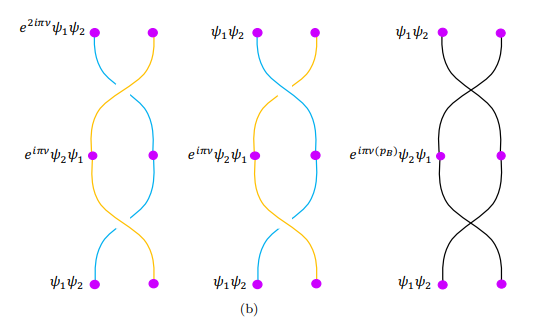
\includegraphics[width=100mm]{braidwf.png}
\caption{ブレイド}
\end{center}
\end{figure}

交換関係を見ると、$\nu=0$でボソンの交換関係を、$\nu=1$でフェルミオンの交換関係を復元することがわかる。
とくに、同じ位置にある粒子においては、エニオニックな位相はキャンセルされ、正準交換関係に帰着する:
\begin{align}
  a(\vb*{x}_\mathcal{C})a^{\dag}(\vb*{x}_\mathcal{C})\pm a^{\dag}(\vb*{x}_\mathcal{C})a(\vb*{x}_\mathcal{C})=1\\
\end{align}
ここで、エニオニックな演算子がフェルミオニックな演算子からきている場合は+、ボソニックな演算子からきている場合は$-$をとる。\\
一般に、トポロジカルエニオンは、$\nu\neq0$のとき、”ハードコアボソン”としてふるまう。ハードコアボソンとは、同じ位置にいない(排他律のある)ボソンである。
この意味で、$\nu$は2つの同一粒子の間の斥力の自由度を定量化していると考えられる。\\
ここの議論は\url{https://www.sciencedirect.com/science/article/pii/055032139390316H}{ A.Lerda, S.Sciuto. Anyons and Quantum Groups}による。

ハードコアボソンの生成消滅演算子$c_i^{\dag}(x_C),c_i(x_C)$を用いて、その議論を追ってみたい。
\begin{align}
  a(\vb*{x}_\mathcal{C})a^{\dag}(\vb*{x}_\mathcal{C})&=K_i(\vb*{x}_C)c_i(\vb*{x})c_i^{\dag}(\vb*{x})K_i^{\dag}(\vb*{x}_C)\\
  &=K_i(\vb*{x}_C)(-c_i^{\dag}(\vb*{x})c_i(\vb*{x})+1)K_i^{\dag}(\vb*{x}_C)\\
  &=-\mathrm{e}^{i\nu\Theta_C(\vb*{x},\vb*{x})}c_i^{\dag}(\vb*{x})K_i(\vb*{x}_c)\mathrm{e}^{i\nu\Theta_C(\vb*{x},\vb*{x})}K_i^{\dag}c_i(\vb*{x})+1\\
  &=-a_i^{\dag}(\vb*{x}_C)a_i(\vb*{x}_C)+1
\end{align}
ただし、
\begin{align}
 K_i(\vb*{x}_C)&=\mathrm{exp}(i\nu\sum_{y\in\Omega}\Theta_{c_{\vb*{x}}}(x,y)c_i^{\dag}(y)c_i(y))\\
K_i^{\dag}(\vb*{x}_C)&=c.c.=K_i^{-1}(\vb*{x}_c)
\end{align}
は、disorder演算子と呼ばれるものである。$\Omega,\Theta$はあとで定義を書くことにする。
これにより中途半端に示された。

\subsection{統計エニオンの第二量子化}
では次に、統計エニオンについて考えよう。
統計エニオンの生成消滅演算子を考えるには、統計エニオンの波動関数を構成したときを思い出せばよい。
量子多体系のHilbert空間として、Fock空間を考える。
そうすると、
\begin{align}
\ket{1}_1\ket{1}_2\dots\ket{1}_N=\prod _{j=1}^{N_B}b_j^{\dag}\ket{0}_j\prod _{k=N_B+1}^{N}f_k^{\dag}\ket{0}_k
\end{align}
と書くことができる。これと同等の表現として統計エニオンの生成演算子を考える:
\begin{align}
  \ket{1}_1\ket{1}_2\dots\ket{1}_N=\prod _{j=1}^{N}s_j^{\dag}\ket{0}_j
\end{align}
演算子$s_j^{\dag}$は、$j\leq N_B$ではボソンの生成演算子に、$N_B\leq j$ではフェルミオンの生成演算子にならなくてはならない。
同様に、消滅演算子も同じ条件を満たさなくてはならない。
この制限のもと、統計エニオンの交換関係は以下のようになる:\\

\begin{itembox}[l]{\textbf{Def.統計エニオンの交換関係 }}
  統計エニオンの交換関係は
\begin{align}
s_j^{\dag}s_j-\mathrm{e}^{i\pi\Theta(j-N_B-1)}s_j s_j^{\dag}=1\\
s_js_j^{\dag}-\mathrm{e}^{i\pi\Theta(j-N_B-1)}s_j^{\dag} s_j=1\\
s_j^{\dag}s_j^{\dag}-\mathrm{e}^{i\pi\Theta(j-N_B-1)}s_j^{\dag} s_j^{\dag}=0\\
s_js_j-\mathrm{e}^{i\pi\Theta(j-N_B-1)}s_j s_j=0
\end{align}
と定義する。
\end{itembox}

1粒子極限を考えると、生成演算子と消滅演算子の関係は

\begin{align}
s_js_j^{\dag}\pm s_j^{\dag}s_j=1
\end{align}

に帰着する。これは、現実にはボソンかフェルミオンかのどちらかであるということを反映している。
また、これは、(5)式の交換関係がフェルミオニックな演算子を元に作られたか、ボソニックな演算子を元に作られたかに依存することを反映している。

\section{統計エニオンと一般化排他統計(Generalized Exclusion Statistics)}
統計エニオンのフェルミオン極限を除いて、統計エニオンとトポロジカルエニオンの注目すべき違いは、排他律がないことである。
かわりに、統計エニオンは”部分的に占有された”状態を許す。
”部分的に占有された状態”というのは、全系の占有率が平均以上の状態である(?)。
この意味で、統計エニオンのフレームワークというのはHaldaneの一般化排他統計(Generalized Exclusion Statistics,GES)に似ている。\\
GESはパウリの排他律を拡張することによって作られたものである。
粒子数を変化させるもとで、量子系のHilbert空間の次元の変化を定量化するパラメタライズされた差分関係(differential relation)を定義することにより拡張された。(この文はまだよくわかっていないのでこんな感じ)
差分関係は

\begin{align}
\Delta  d_{GES}=-g \Delta  N
\end{align}

である。ここで左辺は次元の変化であり、$g$はパラメータだと考えられる。\\
ボソンに対しては、同じ状態を占められる粒子数は無限であるから、次元は粒子数に依存しない。よって$g=0$である。\\
フェルミオンに対しては、排他律のために、それぞれ、追加される粒子によって直接的に次元がスケールされる(粒子がいない次元は考えなくてよいということ?)。よって$g=1$である。\\
GES統計エニオンは、相互作用する気体、たとえばCalogero-Sutherlandモデルなどで見られることが示されている。
驚くべきことに、このGESエニオンの実現は、最低Landau準位に閉じ込められたトポロジカルエニオンに直接マッピングできる。
GESエニオンは、極低温Hubberdチェインと同様に、Calogero-SutherlandモデルやLieb-Linigerモデル、ハードコアTonks-Girardeau気体などに見られている。
もっと一般に、GESに従う理想準粒子の観点から、熱力学的Bethe仮設によって計算しなおせる可積分モデルの存在が示されている。\\
この統計エニオンのフレームワークでは、統計エニオンのHilbert空間の次元変化はボソンの次元変化とフェルミオンの次元変化の和で与えられる。
それぞれの出現確率$p_B,p_F$を用いて、
\begin{align}
\Delta d_{SA}=p_B\Delta d_b+p_F\Delta d_F
\end{align}
とかける。
$\Delta d_B=0,\Delta d_F=-\Delta N$のとき、$\Delta d_{SA}=-p_F\Delta N$と単純になる。
はじめの式と一つ上の式を見比べると、GESのフレームワークにおけるパラメータ$g$というのは、統計エニオンのフレームワークにおけるフェルミオンの出現確率によってきまってしまうということがわかる。
これは統計エニオンのフレームワークがGESエニオンのフレームワークとまったく同等であることを示している。
GESエニオンはボソンとフェルミオンの観点から説明できることは、MurthyとShankerが、Calogero-Sutherlandモデルは理想GESエニオンであることを指摘した際にわかった。
その結果、分配関数はボソニックな部分とフェルミオニックな部分に分けられ、それぞれ、GESパラメータ$g,g-1$の累乗で構成されることがわかった。
これにより、GESはボソンとフェルミオンの理想敵な混合であることが指摘された。\\
統計エニオン、GESエニオンは任意の次元で実現できる(次元に一般的な制限はない)というのは、トポロジカルエニオンとの大きな違いである。


\section{エニオンの平衡熱力学}
\subsection{1次元統計エニオン}
エニオン系の熱力学を理解するためにまず考えることは、熱力学量にエニオンの位相がどのように依存するかである。
これをきめるために、適切な分配関数を導入する。トラップされた相互作用するGESガスの実現でモチベートされたように、1次元調和ポテンシャル中の2つの統計エニオンを考えよう。\\
しかし、この際、我々は相互作用しない粒子系を考えている。
(GESは単なる混合でよいのか?)
トラップされたボソンーフェルミオン混合物は以前より、理論的あるいは実験的に研究されているが、この研究ではおもに、基底状態の設定でボソン、フェルミオン間の相互作用から生じる効果に焦点を当てよう。
統計エニオンのフレームワークでは我々は、混合物の代わりに、そのような混合の理想気体極限として多体平均のふるまいを考える。
調和ポテンシャル中に閉じ込められた2つの統計エニオンのハミルトニアンは

\begin{align}
H=\frac{p_1^2+p_2^2}{2m}+\frac{1}{2}m\omega^2(x_1^2+x_2^2)
\end{align}
で与えられる。統計エニオンののフレームワークでは、ハミルトニアンのもとで発展するエニオンのペアの分配関数というのは
\begin{align}
Z_{SA}=(Z_B)^{p_B}(Z_F)^{1-p_B}
\end{align}
となる。ここで、それぞれの粒子の分配関数を$Z_i,i=B,F$とした。
元論文の付録Aにはこの分配関数の導き方が書いてあるので余裕があるときに読む。$\rightarrow$ これを考えていく。

\subsection{調和ポテンシャル中の統計エニオンの分配関数}
  分配関数は次の様に定義される。ここで、$\ket{x_jy_j}$は位置の固有ケットである。
  \begin{align}
  Z_A^N=\mathrm{tr}{(\mathrm{e}^{-\beta H})}=\prod_{j=1}^N\int dx_j\int dy_j \bra{x_jy_j}\mathrm{e}^{-\beta H_j}\ket{x_j y_j}
  \end{align}
  ここで、
  \begin{align}
  H_j=\frac{p_{x_j}^2+p_{y_j}^2}{2m}+\frac{1}{2}m\omega^2(x_j^2+x_j^2)
  \end{align}
  である。エネルギー固有ケットをアイデンティティとして挟むことによって、位置表示の波動関数$\Psi_A(x_j,y_j)=\braket{n_1^{(j)}n_2^{(j)}}{x_jy_j}$を用いて、
  \begin{align}
  Z_A^N=\prod_{j=1}^N\int dx_j\int dy_j \sum _{n_1^{(j)},n_2^{(j)}} \sum _{m_1^{(j)},m_2^{(j)}} |\Psi_A(x_j,y_j)|^2 \\
  \times \mathrm{e}^{-\beta\hbar\omega(m_1^{(j)}+m_2^{(j)}+1)}\braket{n_1^{(j)}n_2^{(j)}}{m_1^{(j)}m_2^{(j)}} \notag 
  \end{align}
ここで、$\Psi_A(x_j,y_j)$は(4.5)式により定まり、ここでの$\psi$は調和ポテンシャル中の固有関数である。すなわち、
\begin{align}
\psi_n(x)=\frac{1}{\sqrt{2^n n!}}\left(\frac{m\omega}{\pi\hbar}\right)^{\frac{1}{4}}\mathrm{e}^{\frac{m\omega x^2}{2\hbar}}H_n\left(\sqrt{\frac{m\omega}{\hbar}}x\right)  
\end{align}
である($H_n$はエルミート多項式)。
エルミート多項式の直交性を利用することで、
\begin{align}
  Z_A^N=\prod_{j=1}^N \sum _{n_1^{(j)},n_2^{(j)}} \frac{1}{4}\mathrm{e}^{-\beta\hbar\omega(n_1^{(j)}+n_2^{(j)}+1)} \notag \\
  \times (2+\mathrm{e}^{-i\pi\Theta(j-N_B+1)}\delta_{n_1^{(j)},n_2^{(j)}}+\mathrm{e}^{i\pi\Theta (j-N_B+1)}\delta_{n_1^{(j)},n_2^{(j)}})  
\end{align}
積の記号をフェルミオンとボソンに分けることによって、
\begin{align}
  Z_A^N=\prod_{j=1}^{N_B}\sum_{n_1^{(j)},n_2^{(j)}=0}^{\infty}\frac{1}{2}\mathrm{e}^{-\beta\hbar\omega(n_1^{(j)}+n_2^{(j)}+1)}(1+\delta_{n_1^{(j)},n_2^{(j)}})\notag\\
  \times\prod_{k=N_B+1}^{N}\sum_{n_1^{(j)},n_2^{(j)}=0}^{\infty}\frac{1}{2}\mathrm{e}^{-\beta\hbar\omega(n_1^{(j)}+n_2^{(j)}+1)}(1-\delta_{n_1^{(j)},n_2^{(j)}})
\end{align}
これの初めの部分をボソンの分配関数、後半の部分をフェルミオンの分配関数として解釈することができる。
それゆえ、エニオニックな分配関数というのは、このように書ける。
\begin{align}
  Z_A^N=\prod_{j=1}^{N_B}Z_B^{(j)}\prod_{k=1}^{N_F}Z_F^{(k)}=Z_B^{N_B}Z_F^{N_F}=(Z_B^{p_B}Z_F^{p_F})^N
\end{align}
ここで、大きな$N$に対して、$p_B(p_F)$は粒子のペアがボソニック(フェルミオニック)な対称性をもつ確率であり、$N_B=Np_B,N_F=N(1-p_B)$としている。
ボソンとフェルミオンの分配関数はそれぞれ、
\begin{align}
  Z_B=\frac{1}{8}\csch^2\left(\frac{\beta\hbar\omega}{2}\right)+\frac{1}{4}\csch(\beta\hbar\omega)\\
  Z_F=\frac{1}{8}\csch^2\left(\frac{\beta\hbar\omega}{2}\right)-\frac{1}{4}\csch(\beta\hbar\omega)
\end{align}

よって、ひとつの統計エニオンのペアの分配関数は
\begin{align}
  Z_A=\left[\frac{1}{8}\csch^2\left(\frac{\beta\hbar\omega}{2}\right)+\frac{1}{4}\csch(\beta\hbar\omega)\right]^{p_B}\times\left[\frac{1}{8}\csch^2\left(\frac{\beta\hbar\omega}{2}\right)-\frac{1}{4}\csch(\beta\hbar\omega)\right]^{1-p_B}
\end{align}

となる。

この分配関数は、CSmodelの$g\rightarrow1-p_B$としたものに等しい。
我々はここに、統計エニオンの枠組みの中では、エニオニックなふるまいというのは、ハミルトニアンの中の相互作用項からというよりむしろ、平均の性質の上で純粋に現れるということを見ることができる。(CSmodelをもっと見てみる必要があるよこれは)
この分配関数を使うと、熱力学的な量はただちに導かれる。
分配関数を実際に代入してみると、

\begin{align}
E=\frac{1}{2}\hbar \omega[3\coth (\beta\hbar\omega)+\csch(\beta\hbar\omega)-2p_B+1 ]
\end{align}

などとなる。


\section{disscussion}

\subsection{統計エニオンの熱力学量はどのように計測するのか?}
HOM効果の拡張としての統計エニオンの作成は、2つのポート(片方はパスの長さを変えている)から2つのポートへの光子の移動により行われるのであった。
そこから波動関数を考え、分配関数を考え、熱力学量を計算した。
バンチングのあと、統計エニオンはどちらかのポートにいるはずである。
見た目はきっと、単なる光子の集まりであると予想される。
いま、$\nu=\Theta(j-N_B-1)$としているから、$\omega$には影響しない。
よって、なにか周波数に変化が加わることはない。
もし$N_B$に時間依存の項が加わると、周波数が変わったり、波数が変わったりするはずである。





\end{document}
